Il package \textit{gamemanager} rappresenta il controller, responsabile dell'interazione tra model e view, e si compone di:

\begin{itemize}
    \item \textbf{GameManager}: Questo object è l'elemento principale del package e svolge alcune tra le funzioni più importanti relative al controllo logico della partita (come nell'esempio in figura \ref{gameManagerCode}). Viene usato come tramite per la comunicazione tra le classi di model (\textit{GameLogicObserver}) e view (\textit{ViewObserver}), e attraverso esso viene gestita l'inizializzazione della view e il caricamento delle immagini necessarie.
    
    La concorrenza del programma è gestita tramite un approccio basato su task: il loop principale del gioco, \textit{GameLoop}, viene eseguito su un thread separato in uno specifico \textit{ExecutionContext}, mentre altre funzioni che potrebbero richiedere un tempo elevato (caricamento di elementi della view, immagini e suoni) sono delegate a dei thread tramite il meccanismo delle \textit{Future}, che in questo caso vengono eseguite in un \textit{ExecutionContext} fornito da Scala (global). Dovendo gestire proprio questo aspetto, \textit{GameManager} incapsula un \textit{ExecutionContext}, usato per lanciare \textit{GameLoop}, e il valore di \textit{TimeSlice} necessario per la temporizzazione degli step logici del gioco.
    
    \begin{figure}[H]
      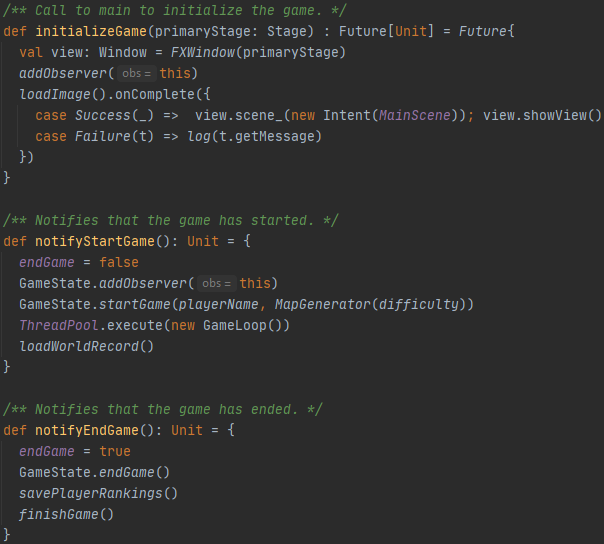
\includegraphics[width=15cm]{res/gameManagerCode.png}
      \caption{Esempio di codice di \textit{GameManager}}
      \label{gameManagerCode}
    \end{figure}

    \item \textbf{GameLoop}: In linea con il design architetturale, questa classe implementa il pattern event-loop per la gestione delle dinamiche di gioco (figura \ref{gameLoopCode}). Come specificato in precedenza, l'event-loop viene lanciato su un thread separato e svolge un ciclo nel quale esegue uno step logico del programma: questo comprende la gestione dei nuovi eventi ed il conseguente aggiornamento della view. Gli eventi vengono inizialmente organizzati in due code, rispettivamente per i movimenti e per gli spari (\textit{playerMoves} e \textit{playerShoots}), per poi essere letti dall'event-loop ad ogni nuovo step.
    
    \begin{figure}[H]
      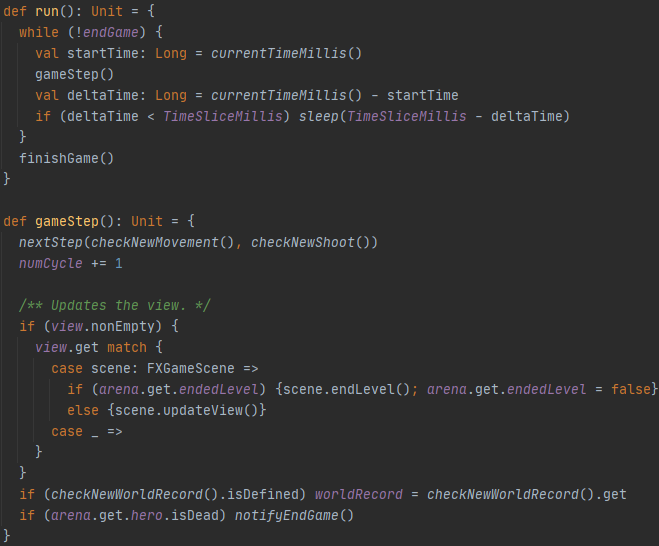
\includegraphics[width=15cm]{res/gameLoopCode.png}
      \caption{Esempio di codice di \textit{GameLoop}}
      \label{gameLoopCode}
    \end{figure}

    \item \textbf{ViewObserver}: Interfaccia che rappresenta l'observer della view nell'implementazione del pattern Observer. Viene utilizzata per la comunicazione da view a controller e si occupa di notificare le transizioni tra le varie scene; inoltre, notifica i \textit{KeyEvent} generati dall'utente e catturati dalla \textit{GameView}. Quando un evento viene notificato, viene aggiunto alla relativa coda per essere successivamente consumato dal \textit{GameLoop}, come riportato in figura \ref{notifyAction}.
    
    \begin{figure}[H]
      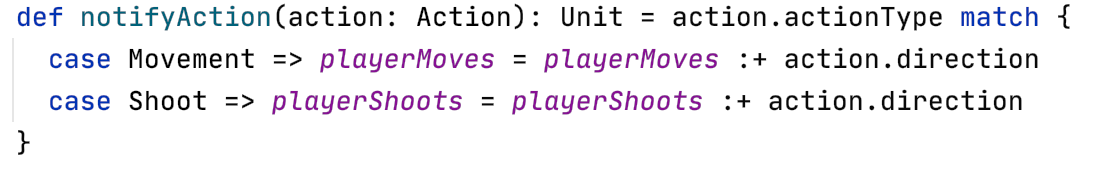
\includegraphics[width=14cm]{res/notifyAction.png}
      \caption{Aggiunge l'azione notificata alla relativa coda}
      \label{notifyAction}
    \end{figure}
\end{itemize}